% !TeX program = pdflatex
\documentclass[oneside,a4paper,14pt]{extarticle}
\usepackage[T1,T2A]{fontenc}
\usepackage[
a4paper,
letterpaper,
top=2cm,
bottom=2cm,
left=2.5cm,
right=1.5cm
]{geometry}
\usepackage[utf8]{inputenc}
\usepackage[russian]{babel}
\usepackage{textcomp}
\usepackage{indentfirst}
\usepackage{listings}
\usepackage{xcolor}
\usepackage{enumitem}
\usepackage{graphicx}
\usepackage{mwe}
\usepackage{wrapfig}
\usepackage{caption}
\usepackage{amsmath}
\usepackage{amsfonts}
\usepackage{float}
\usepackage{amsthm}
\usepackage[all]{xy}
\usepackage[breaklinks]{hyperref}
\usepackage{titlesec}
\usepackage{adjustbox}
\usepackage{tikz}
\usetikzlibrary{positioning,arrows.meta,shapes.multipart}

\titleformat{\section}
{\normalsize\bfseries}
{\thesection} {1em}{}
\titleformat{\subsection}
{\normalsize\bfseries}
{\thesubsection} {1em}{}
\titleformat{\subsubsection}
{\normalsize\bfseries}
{\thesubsubsection} {1em}{}
\renewcommand\baselinestretch{1.33}
\normalsize
\setlength{\parindent}{1.25cm}

\lstset{
	language=Python,
	basicstyle=\ttfamily\small,
	keywordstyle=\color{blue},
	commentstyle=\color{green!60!black},
	stringstyle=\color{red},
	numbers=left,
	numberstyle=\tiny\color{gray},
	frame=single,
	breaklines=true,
	showstringspaces=false,
	tabsize=4,
	inputencoding=utf8,
	extendedchars=true,
	literate={а}{{\selectfont\char224}}1 {б}{{\selectfont\char225}}1 {в}{{\selectfont\char226}}1 {г}{{\selectfont\char227}}1 {д}{{\selectfont\char228}}1 {е}{{\selectfont\char229}}1 {ё}{{\"e}}1 {ж}{{\selectfont\char230}}1 {з}{{\selectfont\char231}}1 {и}{{\selectfont\char232}}1 {й}{{\selectfont\char233}}1 {к}{{\selectfont\char234}}1 {л}{{\selectfont\char235}}1 {м}{{\selectfont\char236}}1 {н}{{\selectfont\char237}}1 {о}{{\selectfont\char238}}1 {п}{{\selectfont\char239}}1 {р}{{\selectfont\char240}}1 {с}{{\selectfont\char241}}1 {т}{{\selectfont\char242}}1 {у}{{\selectfont\char243}}1 {ф}{{\selectfont\char244}}1 {х}{{\selectfont\char245}}1 {ц}{{\selectfont\char246}}1 {ч}{{\selectfont\char247}}1 {ш}{{\selectfont\char248}}1 {щ}{{\selectfont\char249}}1 {ъ}{{\selectfont\char250}}1 {ы}{{\selectfont\char251}}1 {ь}{{\selectfont\char252}}1 {э}{{\selectfont\char253}}1 {ю}{{\selectfont\char254}}1 {я}{{\selectfont\char255}}1 {А}{{\selectfont\char192}}1 {Б}{{\selectfont\char193}}1 {В}{{\selectfont\char194}}1 {Г}{{\selectfont\char195}}1 {Д}{{\selectfont\char196}}1 {Е}{{\selectfont\char197}}1 {Ё}{{\"E}}1 {Ж}{{\selectfont\char198}}1 {З}{{\selectfont\char199}}1 {И}{{\selectfont\char200}}1 {Й}{{\selectfont\char201}}1 {К}{{\selectfont\char202}}1 {Л}{{\selectfont\char203}}1 {М}{{\selectfont\char204}}1 {Н}{{\selectfont\char205}}1 {О}{{\selectfont\char206}}1 {П}{{\selectfont\char207}}1 {Р}{{\selectfont\char208}}1 {С}{{\selectfont\char209}}1 {Т}{{\selectfont\char210}}1 {У}{{\selectfont\char211}}1 {Ф}{{\selectfont\char212}}1 {Х}{{\selectfont\char213}}1 {Ц}{{\selectfont\char214}}1 {Ч}{{\selectfont\char215}}1 {Ш}{{\selectfont\char216}}1 {Щ}{{\selectfont\char217}}1 {Ъ}{{\selectfont\char218}}1 {Ы}{{\selectfont\char219}}1 {Ь}{{\selectfont\char220}}1 {Э}{{\selectfont\char221}}1 {Ю}{{\selectfont\char222}}1 {Я}{{\selectfont\char223}}1 {«}{{\guillemotleft}}1 {»}{{\guillemotright}}1 {№}{{\textnumero}}1 {–}{{--}}1,
}

\begin{document}
	\sloppy
	\newpage\thispagestyle{empty}
	\begin{center}
		МИНИСТЕРСТВО НАУКИ И ВЫСШЕГО ОБРАЗОВАНИЯ\\
		РОССИЙСКОЙ ФЕДЕРАЦИИ\\
		ФЕДЕРАЛЬНОЕ ГОСУДАРСТВЕННОЕ БЮДЖЕТНОЕ\\
		ОБРАЗОВАТЕЛЬНОЕ УЧРЕЖДЕНИЕ ВЫСШЕГО ОБРАЗОВАНИЯ\\
		<<ВЯТСКИЙ ГОСУДАРСТВЕННЫЙ УНИВЕРСИТЕТ>>\\
		Институт математики и информационных систем\\
		Факультет автоматики и вычислительной техники\\
		Кафедра электронных вычислительных машин
	\end{center}
	\vspace{20mm}
	\begin{center}
		Отчёт по лабораторной работе №1\\
		по дисциплине\\
		<<Теория автоматов>>
	\end{center}
	\vspace{40mm}
	\noindent
	Выполнил студент гр. ИВТб-2303 \hfill \rule[-0,5mm]{30mm}{0.15mm}\,/Шубин В. Ю./
	\newline
	Проверил преподаватель кафедры ЭВМ \hfill \rule[-0,5mm]{30mm}{0.15mm}\,/Мельцов В. Ю./
	\vfill
	\begin{center}
		Киров\\
		2026
	\end{center}
	\newpage
	\thispagestyle{empty}
	\section*{Цель работы:} Создать автомат по заданному ТЗ. Оформить схему алгоритма и разработать приложение на языке Python с графическим интерфейсом, реализующее алгоритм автомата. Продемонстрировать работу программы.

	\section*{Среда разработки:} Python 3.12, стандартные модули \texttt{tkinter} и \texttt{ttk}, редактор Visual Studio Code.

	\newpage
	
	\section*{1. Постановка задачи и схема алгоритма}
	
	На экране отображаются пять окружностей разных цветов. Программа случайным образом генерирует координаты точки (звёздочки) и определяет, попала ли она в какую-либо окружность. Если попадание произошло, счётчик этой окружности увеличивается на единицу. Когда счётчик достигает значения 10, окружности присуждается место, которое она заняла по сбору звёздочек (первая заполненная --- 1-е место, вторая --- 2-е и так далее). После того как все пять окружностей набрали по 10 точек, программа завершает работу.
	
	
	Полная схема алгоритма приведена на рисунке~1.
	
	\begin{figure}[H]
		\centering
		\adjustbox{max width=0.95\linewidth}{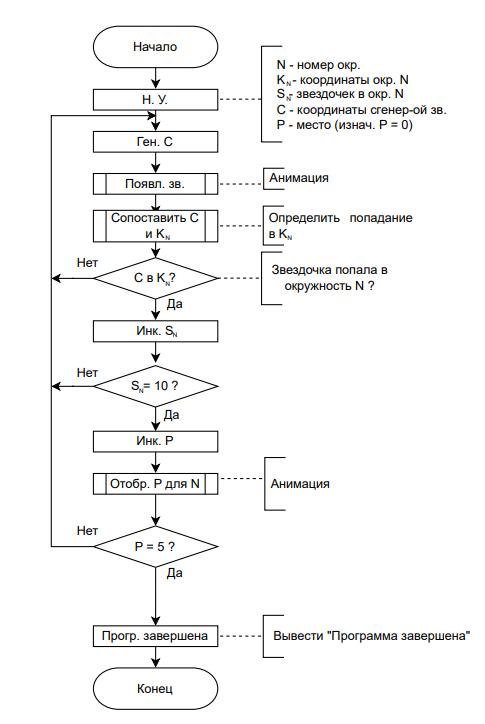
\includegraphics{схематавт1.png}}
		\caption{Схема алгоритма работы программы}
	\end{figure}
	
	\newpage
	
	\section*{2. Структура программы и описание функций}
	
	Программа представляет собой один модуль, в котором находятся все элементы интерфейса и логика. Основные функции и их назначение приведены в таблице~1.
	
	\begin{table}[H]
		\centering
		\small
		\caption{Основные функции программы}
		\begin{tabular}{|p{4.6cm}|p{10.4cm}|}
			\hline
			\textbf{Функция} & \textbf{Назначение}\\
			\hline
			\texttt{get\_points\_in\_circle} & Формирует множество целочисленных координат, принадлежащих окружности с центром $(cx, cy)$ и радиусом $r$.\\
			\hline
			\texttt{draw\_star} & Рисует звездочку в заданной точке холста (четыре линии).\\
			\hline
			\texttt{lighten\_color} & Получает светлый оттенок цвета для заливки завершённой окружности.\\
			\hline
			\texttt{show\_speed\_error} & Показывает временное окно ошибки ввода скорости с уменьшением времени показа при повторах.\\
			\hline
			\texttt{save/load\_colors\_to/from\_file} & Сохранение и загрузка пяти названий цветов в текстовом файле.\\
			\hline
			\texttt{open\_color\_dialog} & Диалог выбора уникального цвета для каждой из пяти окружностей.\\
			\hline
			\texttt{about\_program}, \texttt{about\_author} & Вывод справки о программе и об авторе.\\
			\hline
			\texttt{update\_layout}, \texttt{draw\_initial\_scene} & Пересчёт геометрии при изменении размера окна и отрисовка начальной сцены.\\
			\hline
			\texttt{generate\_step} & Шаг алгоритма: генерация точки, проверка попадания, обновление счётчика, места и заливки.\\
			\hline
			\texttt{reset\_state}, \texttt{start\_program}, \texttt{pause\_program}, \texttt{resume\_program} & Управление игрой: сброс, запуск/стоп, пауза и продолжение.\\
			\hline
			\texttt{on\_scale\_change}, \texttt{on\_entry\_change}, \texttt{update\_speed} & Работа с ползунком и полем ввода скорости (0--100).\\
			\hline
		\end{tabular}
	\end{table}
	
	Приложение имеет меню «Файл» (Открыть, Сохранить), «Настройки» (Цвет) и «Помощь» (О программе, Об авторе). Справа расположены кнопки «Старт/Стоп», «Пауза/Продолжить», «Выход» и ползунок скорости с полем ввода.
	
	\newpage
	
	\section*{3. Основные фрагменты исходного кода}
	
	\subsection*{Геометрия и отрисовка}
	\begin{lstlisting}[language=Python]
def get_points_in_circle(cx, cy, r):
    points = []
    r_sq = r * r
    for x in range(math.floor(cx - r), math.floor(cx + r) + 1):
        dx = x - cx
        dy_sq = r_sq - dx * dx
        if dy_sq >= 0:
            dy = math.sqrt(dy_sq)
            for y in range(math.floor(cy - dy), math.floor(cy + dy) + 1):
                points.append((x, y))
    return points

def draw_initial_scene():
    global counter_labels, ranking_labels, circle_oval_ids
    counter_labels = []
    ranking_labels = []
    circle_oval_ids = []
    for i, (cx, cy) in enumerate(circles_coords):
        oval_id = canvas.create_oval(cx - RADIUS, cy - RADIUS,
                                     cx + RADIUS, cy + RADIUS,
                                     outline=circle_colors[i], width=2)
        circle_oval_ids.append(oval_id)
        canvas.create_oval(cx - 3, cy - 3, cx + 3, cy + 3,
                           fill=circle_colors[i], outline=circle_colors[i])
    for i, (cx, cy) in enumerate(circles_coords):
        label = canvas.create_text(cx, cy - 20, text="0/10",
                                   fill=circle_colors[i], font=("Arial", 10, "bold"))
        counter_labels.append(label)
        rank_label = canvas.create_text(cx, cy - 40, text="",
                                        fill=circle_colors[i], font=("Arial", 10, "bold"))
        ranking_labels.append(rank_label)
	\end{lstlisting}
	
	\subsection*{Шаг алгоритма}
	\begin{lstlisting}[language=Python]
def generate_step():
    global running, paused, p, after_id, finished
    if not running or paused: return
    x = rand.randint(0, canvas.winfo_width() - 1)
    y = rand.randint(0, canvas.winfo_height() - 1)
    c = (x, y)
    hit = False
    for i in range(5):
        if c in all_coords[i]:
            if s[i] < 10:
                s[i] += 1
                draw_star(canvas, x, y, size=3, color=circle_colors[i])
                canvas.itemconfig(counter_labels[i], text=f"{s[i]}/10")
                if s[i] == 10:
                    canvas.itemconfig(circle_oval_ids[i],
                                      fill=lighten_color(circle_colors[i]))
                    canvas.itemconfig(ranking_labels[i], text=f"Место: {p}")
                    p += 1
                    if p == 6:
                        running = False
                        finished = True
                        if after_id is not None:
                            root.after_cancel(after_id)
                            after_id = None
                        menubar.entryconfigure(SETTINGS_MENU_INDEX, state="disabled")
                        messagebox.showinfo("Завершено", "Программа завершена")
                        return
            else:
                draw_star(canvas, x, y, size=3, color="gray")
            hit = True
            break
    if not hit:
        draw_star(canvas, x, y, size=3, color="gray")
    root.update()
    after_id = root.after(current_delay, generate_step)
	\end{lstlisting}
	
	\subsection*{Управление игрой}
	\begin{lstlisting}[language=Python]
def reset_state():
    global p, s, running, paused, finished, after_id, counter_labels, ranking_labels
    if after_id is not None:
        root.after_cancel(after_id)
        after_id = None
    running = False
    paused = False
    finished = False
    p = 1
    s = [0, 0, 0, 0, 0]
    canvas.delete("all")
    if circles_coords:
        draw_initial_scene()
    btn_start.config(text="Старт", command=start_program)
    btn_pause.config(text="Пауза", command=pause_program, state=tk.NORMAL)
    menubar.entryconfigure(SETTINGS_MENU_INDEX, state="normal")

def start_program():
    global running, paused, finished
    if finished: return
    running = True
    btn_start.config(text="Стоп", command=reset_state)
    menubar.entryconfigure(SETTINGS_MENU_INDEX, state="disabled")
    if not paused:
        btn_pause.config(text="Пауза", command=pause_program, state=tk.NORMAL)
    generate_step()

def pause_program():
    global paused
    paused = True
    btn_pause.config(text="Продолжить", command=resume_program)

def resume_program():
    global paused, after_id
    paused = False
    btn_pause.config(text="Пауза", command=pause_program)
    if running and not finished:
        if after_id is not None:
            root.after_cancel(after_id)
            after_id = None
        generate_step()
	\end{lstlisting}
	
	\subsection*{Контроль скорости ввода}
	\begin{lstlisting}[language=Python]
def on_entry_change(event=None):
    global last_valid_speed, updating
    if updating: return
    updating = True
    try:
        value = speed_var.get()
        if value == "":
            if last_valid_speed == "0":
                entry.delete(0, tk.END)
                entry.insert(0, "0")
                entry.icursor(tk.END)
                return
            else:
                scale.set(0)
                update_speed(0)
                return
        if not value.isdigit():
            show_speed_error("Ошибка", "Недопустимый символ", "not_digit")
            entry.delete(0, tk.END)
            entry.insert(0, last_valid_speed)
            return
        if value.startswith("0") and len(value) > 1:
            show_speed_error("Ошибка", "Незначащие нули удалены",
                             "leading_zero_removed")
            new_value = value.lstrip("0") or "0"
            entry.delete(0, tk.END)
            entry.insert(0, new_value)
            last_valid_speed = new_value
            scale.set(int(new_value))
            update_speed(int(new_value))
            return
        num = int(value)
        if num > 100:
            show_speed_error("Ошибка", "Вводите числа от 0 до 100", "max_speed")
            entry.delete(0, tk.END)
            entry.insert(0, "100")
            last_valid_speed = "100"
            scale.set(100)
            update_speed(100)
            return
        last_valid_speed = value
        scale.set(num)
        update_speed(num)
    finally:
        updating = False
	\end{lstlisting}
	
	\newpage
	
	\section*{4. Экранные формы работы приложения}
	
	После запуска программы отображается главное окно с пятью окружностями, окрашенными в начальные цвета (рисунок~2). Над каждой окружностью выводится счётчик вида «0/10», ниже --- место (пока пустое). Справа расположены кнопки управления и ползунок скорости.
	
	\begin{figure}[H]
		\centering
		\adjustbox{max width=0.92\linewidth}{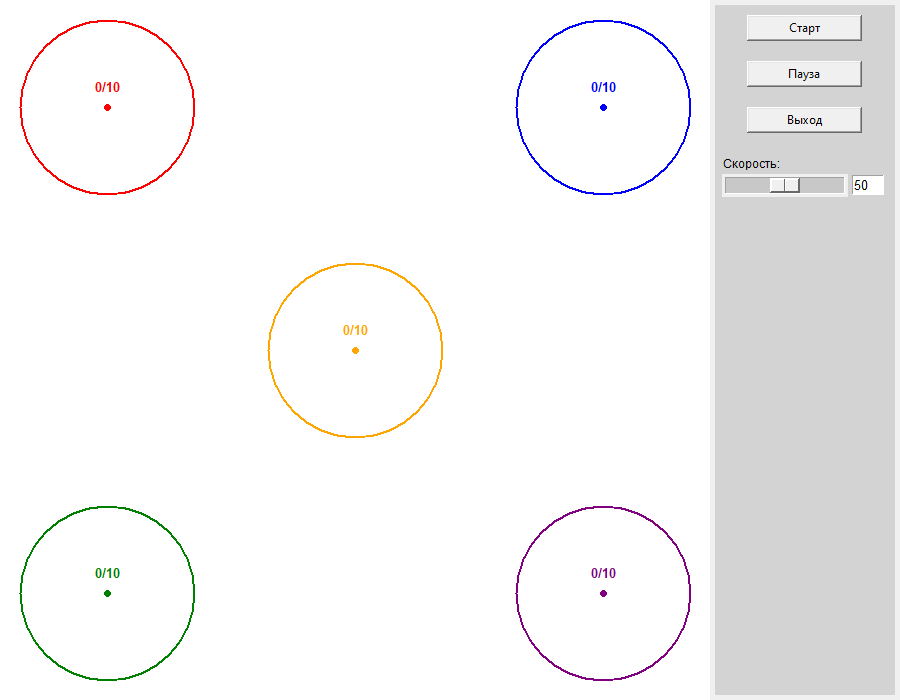
\includegraphics{s1.png}}
		\caption{Главное окно программы сразу после запуска}
	\end{figure}
	
	Диалог «Настройки --- Цвет» показан на рисунке~3. Список цветов отсортирован по алфавиту. Справа от каждого названия расположен цветной квадратик.
	
	\begin{figure}[H]
		\centering
		\adjustbox{max width=0.92\linewidth}{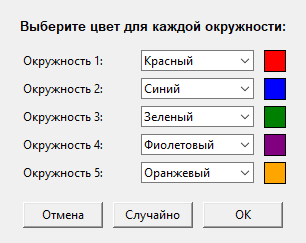
\includegraphics{s2.png}}
		\caption{Диалог выбора цветов окружностей}
	\end{figure}
	
	При попытке выбрать один и тот же цвет для двух окружностей выводится короткое сообщение «Этот цвет уже выбран» (рисунок~4).
	
	\begin{figure}[H]
		\centering
		\adjustbox{max width=0.92\linewidth}{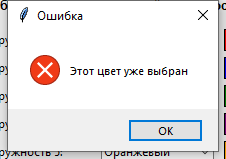
\includegraphics{s3.png}}
		\caption{Сообщение о повторном выборе цвета}
	\end{figure}
	
	При вводе в поле скорости значения больше 100 появляется подсказка «Вводите числа от 0 до 100», после чего поле автоматически принимает значение 100 (рисунок~5).
	
	\begin{figure}[H]
		\centering
		\adjustbox{max width=0.92\linewidth}{
\includegraphics{s4.png}}
		\caption{Сообщение при вводе скорости больше 100}
	\end{figure}
	
	Справка «О программе» представлена на рисунке~6. Текст содержит описание кнопок, скорости, цветов, сохранения файла и изменения размера окна.
	
	\begin{figure}[H]
		\centering
		\adjustbox{max width=0.92\linewidth}{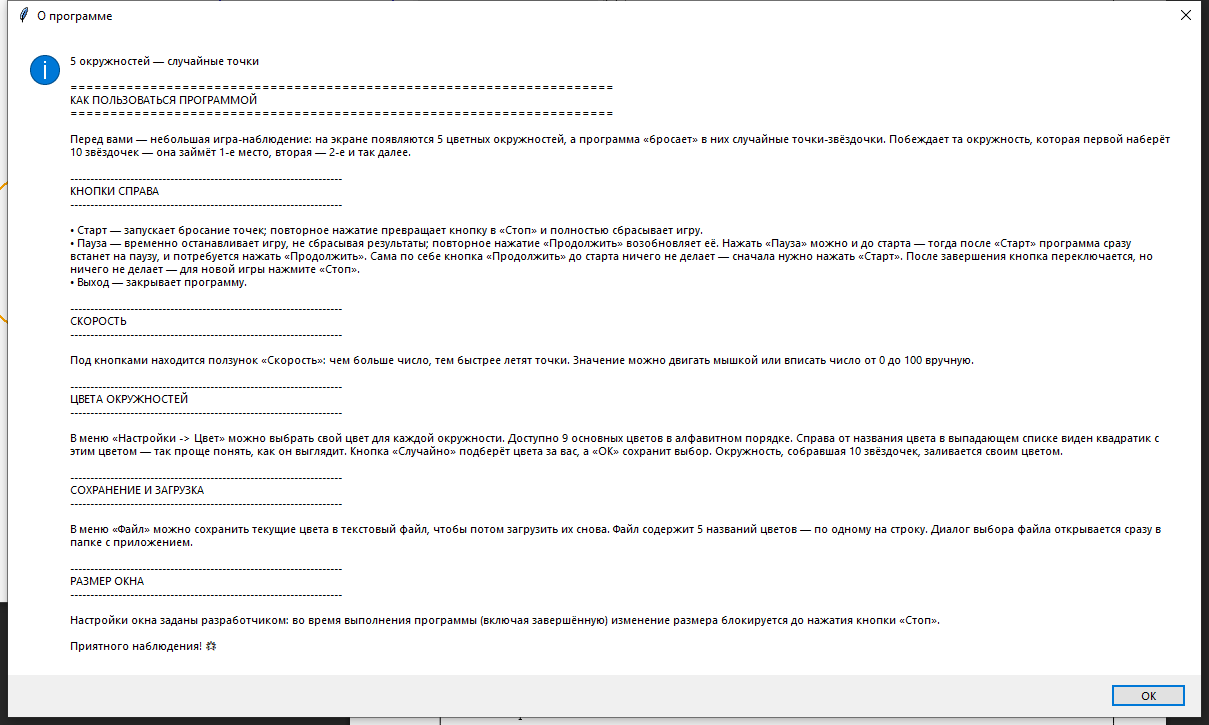
\includegraphics{s5.png}}
		\caption{Справка «О программе» с расширенным текстом}
	\end{figure}
	
	Справка «Об авторе» содержит сведения об исполнителе работы (рисунок~7).
	
	\begin{figure}[H]
		\centering
		\adjustbox{max width=0.92\linewidth}{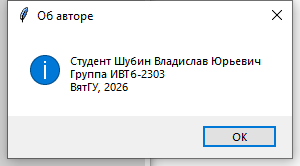
\includegraphics{s6.png}}
		\caption{Справка «Об авторе»}
	\end{figure}
	
	В процессе работы (рисунок~8) программа генерирует звёздочки в случайных координатах; попавшие в окружность окрашиваются в её цвет, остальные --- в серый. Счётчики постепенно увеличиваются.
	
	\begin{figure}[H]
		\centering
		\adjustbox{max width=0.92\linewidth}{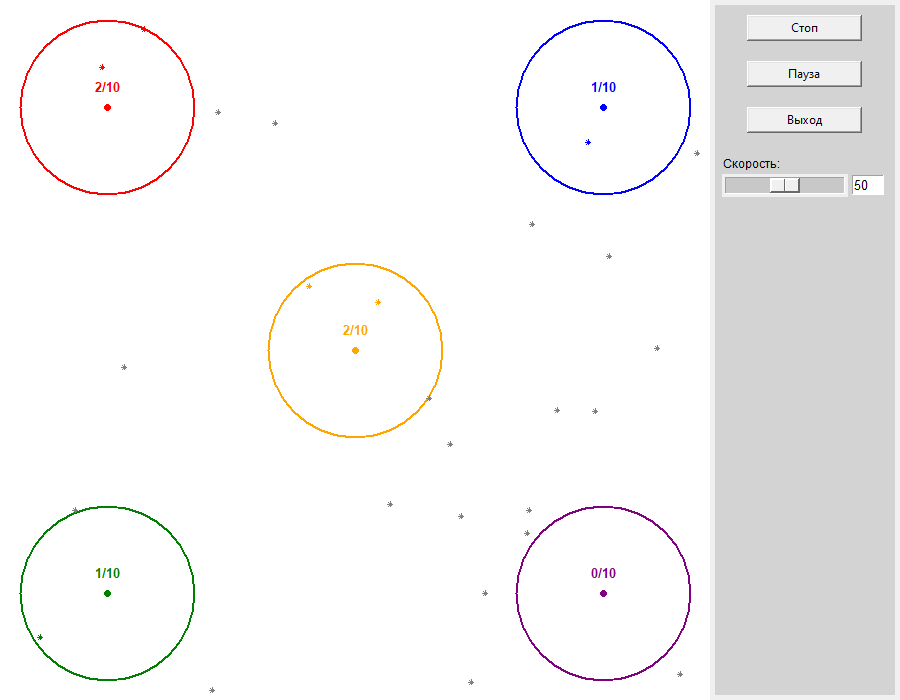
\includegraphics{s7.png}}
		\caption{Процесс генерации точек и заполнения окружностей}
	\end{figure}
	
	Когда окружность набирает 10 точек, она заливается светлым оттенком своего цвета, а под счётчиком появляется занятое место (рисунок~9).
	
	\begin{figure}[H]
		\centering
		\adjustbox{max width=0.92\linewidth}{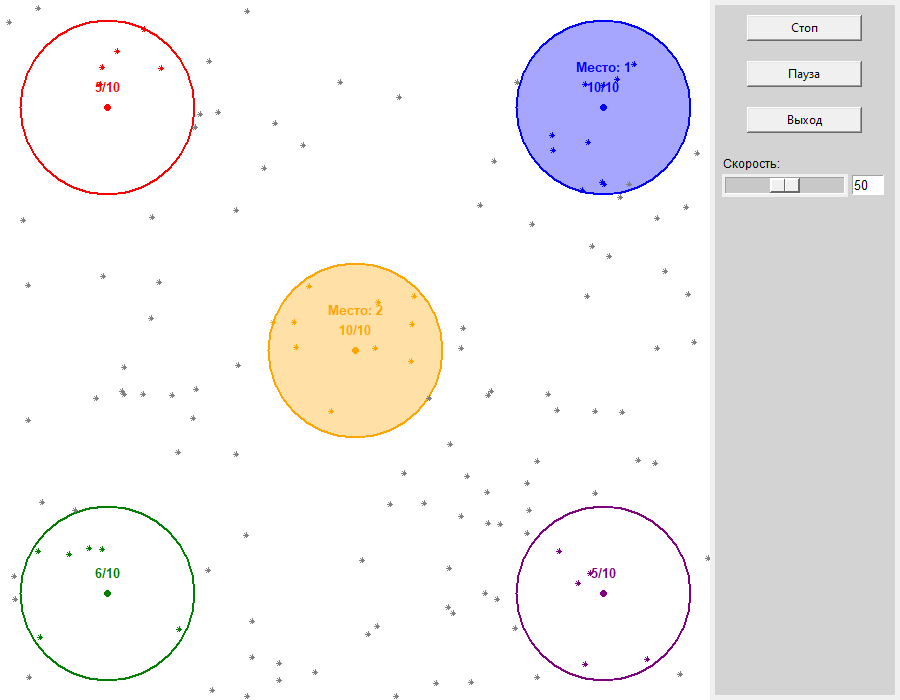
\includegraphics{s8.png}}
		\caption{Заливка окружностей после набора 10 точек}
	\end{figure}
	
	После заполнения всех пяти окружностей появляется сообщение «Программа завершена» (рисунок~10).
	
	\begin{figure}[H]
		\centering
		\adjustbox{max width=0.92\linewidth}{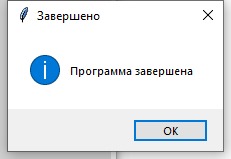
\includegraphics{s9.png}}
		\caption{Сообщение о завершении работы программы}
	\end{figure}
	
	Вид завершённой игры после закрытия сообщения показан на рисунке~11: все окружности залиты, занятые места выведены над счётчиками.
	
	\begin{figure}[H]
		\centering
		\adjustbox{max width=0.92\linewidth}{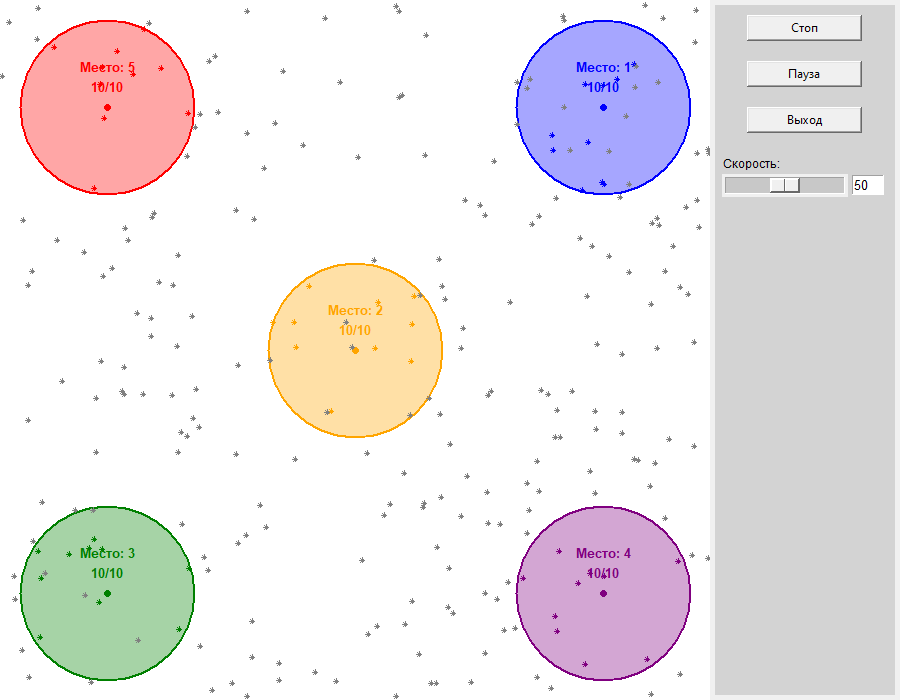
\includegraphics{s10.png}}
		\caption{Итоговое состояние игры}
	\end{figure}
	
	\newpage
	
	\section*{Выводы} В ходе выполнения лабораторной работы был успешно создан автомат по ТЗ и разработана программа на языке Python с графическим интерфейсом на базе \texttt{tkinter}, реализующая алгоритм случайного выпадения звёздочек в пять окружностей. Построена схема алгоритма в соответствии с заданием (рисунок~1). Реализованы генерация точек, подсчёт попаданий, определение мест, заливка завершённых окружностей, пауза и сброс, выбор цветов, сохранение и загрузка настроек, а также контроль ввода скорости. Работа программы продемонстрирована на скриншотах (рисунки~2--11).
	
\end{document}
